%!TEX root = ../PhDthesis.tex
\chapter{Modelling the effects of visual statistics on long-range lateral connectivity in visual cortex}

One of the major problems in computational neuroscience is in
understanding how the brain can robustly capture information about its
environment to improve how new information is encoded and
processed. One of the major benefits of the developmental models such
as those developed in the previous chapters is that the developed
synaptic connections reflect the visual statistics of the
input. Therefore we can make predictions about how the statistics
embedded in the visual inputs is reflected in the organization of the
model and could be used to aid cortical computations.

A number of studies have investigated the role visual statistics play
in shaping the organization of cortex. In particular it has been shown
that the distribution of orientations in the orientation maps can be
strongly affected by altering the visual experience of an animal
through manipulations like goggle rearing \cite{Tanaka2006}. However
the evidence for the encoding of second-order statistics in lateral
connections has been much harder to study and even coarse approaches
such as measuring the isotropy of lateral connections along the axis
of preferred orientation has not yielded uniform results. While a
number of studies have found that lateral connections are elongated
along the axis of preferred orientation in tree shrew
\citep{Bosking1997}, cat \citep{Schmidt1997} and owl monkey
\citep{Sincich2001} in macaque this anisotropy could be explained by
the anisotropy in cortical magnification such that the connections are
not elongated in visual space \citep{Angelucci2002}.  Whether this
reflects differences in rearing environments or actual species
differences is not fully clear, as the tracer injections required to
reconstruct the lateral connections can be performed at most on a few
cells in a single animal, making the collection of a lot of data
infeasible.

Although there is a clear lack of data in this area a few attempts
have been made to go further and establish whether the lateral
projections connect co-circular orientation domains, relecting the
co-circularity in natural images \citep{Hunt2011}. These studies have
again been inconclusive due to the sparsity of good quality data.

In this chapter we will employ the model introduced in the previous
chapter to analyze to what extent the statistics of the visual input
shape the long-range excitatory connections and attempt to reconstruct
those statistics based purely on synaptic weights and orientation
map. In doing so we will determine to what extent they can capture the
statistics of the training dataset and establish whether considerable
biases in the inputs could affect the isotropy of connections.

\section{Methods}

\subsubsection{Synthetic stimuli}

The stimuli generated for this purpose are simple extensions of the
elongated 2D Gaussian stimuli used to train the models up to this
point. The model will draw 1 stimulus per unit area, which consists of
a chain of three Gaussian pattern, the patterns can be seen in
\ref{GaussianStatistics}. The middle Gaussian determines the overall
orientation ($\theta_M$) of the pattern, and the outer Gaussians are
offset in orientation by a value drawn from a vonMises distribution
with a mean of $\theta_M$ and a $\kappa$ of ${0.5, 2, 8}$. The
patterns are then spatially offset so that they form a chain forming
either 'S' shaped or 'U' shaped providing circular and anti-circular
statistics respectively. By varying the $\kappa$ we can vary how the
distribution of co-occurence statistics increasing the preference for
simple elongated bars.

\begin{figure}
	\centering
	\includegraphics[width=1.0\textwidth]{./results/lespi/gaussian_statistics.pdf}
	\caption[Example of Gaussian patterns with co-occurence
      statistics] {Gaussian patterns with co-occurence statistics
      where the orientation offset is drawn from a vonMises
      distribution with different $\kappa$ values and either co- or
      anti-circular statistics.}
    \label{GaussianStatistics}
\end{figure}

\subsection{Weight Isotropy}

The isotropy of the long-range projecting lateral excitatory
projections was analyzed by computing the angle between the
post-synaptic cells' preferred orientation and the pre-synaptic cell
location and was then binned into a polar histogram. This provides a
simple measure of whether the weights are anisotropic along the axis
of preferred orientation of a neuron.

Additionally we will test explicitly whether the lateral connections
are elongated along the axis of preferred orientation by fitting the
\cite{Buzas2006} model of lateral connectivity leaving the orientation
component as a free parameter. This will provide twofold validation,
whether the model is actually connects to neurons nearby in the
orientation domain but also allow us to estimate the aspect ratio of
the connectivity.

\subsection{Second order statistics}

The afferent receptive fields in the visual cortex are usually assumed
to act as feature detectors reducing the dimensionality of the visual
``pixel`` space into a lower dimensional representation. Connections
between these feature detectors could therefore at least in theory
represent the co-occurence statistics of the low level features. In
primary visual cortex this would just represents the co-occurence of
simple oriented edges.

In a recent paper \cite{Perrinet2015} analyzed the edge co-occurence
statistics in natural images by labeling images with edges at varying
frequencies, scales, orientations and phases through a greedy
algorithm and then computing both the relative orientation between
each pair of edges and the normalized azimuthal angle between them. An
example image with labeled edges is shown in \ref{classifier}, along
with a diagram showing how the co-occurence were computed.

\begin{figure}
	\centering
    \includegraphics[width=0.8\textwidth]{./classifier.pdf}
	\caption[] {Diagramatic representation of how a classifier is
      trained to distinguish between natural images and inanimate
      objects. A) The different layers used to train the
      classifier. The natural images are first fed through a model
      retina, all the edges are labeled with positions and
      scales. Using a greedy algorithm a set of edges accounting for
      the largest amount of luminance variance within the original
      image are selected. Using this set of edges the edge
      co-occurence statistics were computed and finally the classifier
      was trained based on these statistics. B) The sparse set
      of labelled edges extracted from a single image. C) Diagram
      showing how the angular difference $\theta$ and azimuth angle
      $\phi$ and relative azimuth $\psi$ are computed from two
      edges. Reproduced from \cite{Perrinet2015}.}
	\label{classifier}
\end{figure}

This method for computing the edges was applied to the lateral
connection fields of the LESPI model trained on a variety of
stimuli. This was done by computing both the relative orientation and
azimuth between each pre- and post-synaptic set of neurons and then
binning these statistics weighted by the strength of connections
between them as well as the orientation selectivity of both neurons.

The lateral connection fields were chosen by selecting regions with a
high local homogeneity index suggesting that the neuron is located in
a iso-orientation domain. This matches the protocol employed by
\cite{Bosking1997}, who chose 13 neurons in the center of orientation
domains.

\subsection{Training stimuli}

The first step was to train the model on the different image datasets,
which had already been analyzed for their co-occurence statistics (see
figure \ref{classifier}). The datasets fed to the model comprised the
two datasets used as part of the paper and one additional image
dataset recorded in treeshrew cages in the David Fitzpatrick lab at
Duke University, which features great numbers of extended,
high-contrast bars (shown in figure \ref{datasets}).

\begin{figure}
	\centering
	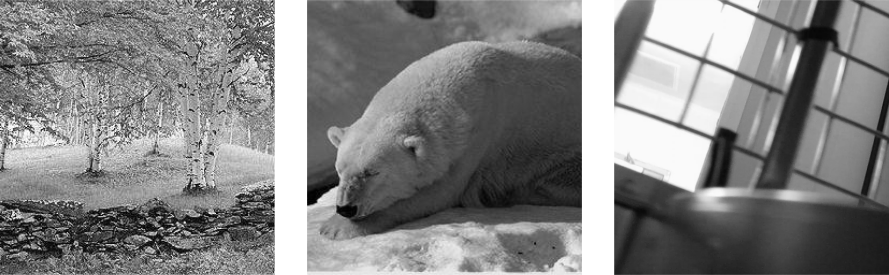
\includegraphics[width=1.0\textwidth]{./image_datasets.pdf}
	\caption[]%
            {The three image datasets used to train the model. From
      left to right 1) Artificial dataset 2) Animal dataset 3) Ferret
      cage dataset.}
    \label{datasets}
\end{figure}

\section{Results}

It was found that for the distances that are contained within one
lateral field there was very little difference when binning the data
separately, which matches the fact that the classifier employed by
\cite{Perrinet2015} could extract little information from the
distance. In order to reduce the local contribution the central
weights within the same microcolumn were masked out. The resultant
plots are shown in figure \ref{cooccurrence}. Generally a good match
is found between the co-occurence statistics in the dataset and the
statistics encoded in the long-range connections of the model. The
difference is clearest when comparing the laboratory dataset to the
natural dataset, likely because the statistics are so radically
different between these datasets.

\begin{figure}
	\centering
        \includegraphics[width=1.0\textwidth]{cooccurrence_plots.pdf}
	\caption{Co-occurence histograms comparing the distribution of
          orientation and relative azimuth of edges extracted from two
          image datasets and the equivalent distribution extracted
          from the lateral connection patterns of the LESPI model,
          highlighting that the model was able to capture the most
          characteristic features of this dataset.}
	\label{cooccurrence}
\end{figure}


\begin{itemize}
\item First order orientation distribution
\item Describe Buzas fitting process
\item Describe decoding orientation and azimuth histograms from lateral
  connectivity
\item Describe anisotropy results for different datasets
\item Discuss further work including:
\item Better decoding of position preference
\item Include orientation selectivity in Buzas model
\end{itemize}



\section{Discussion}

* 
